\subsection{Frontend}
Ogni volta che la pagina viene caricata, viene chiamato uno \texttt{useEffect}.
Lo \texttt{useEffect} è un hook di React che viene eseguito quando il componenete viene montato nel DOM. \cite{reactUseEffect}
\begin{lstlisting}[language=typescript, frame=lines, basicstyle=\ttfamily\scriptsize, numbers=left]
useEffect(() => {
    const jwtToken = TokenAuth.getTokenAuth();
    
    const getMeet = async () => {
        try {
           const response = await ritornaMeeting(jwtToken);
           setEvents(response.data);
        } catch (error) {
           setPopupBackgroundColor('red');
           showPopup('Errore durante il caricamento dei colloqui');
           console.error('Errore durante il recupero degli eventi:', error);
        }
    };  
    getMeet();
}, []);
\end{lstlisting}
\begin{itemize}
    \item \textbf{Riga 2}: viene recuperato il \texttt{jwtToken} dell'utente. Abbreviazione di \textbf{JSON Web Token}, 
    il \texttt{jwtToken} è uno standard (RFC 7519) per trasmettere in modo sicuro dei dati sotto forma di oggeto JSON. \cite{jwtToken}
    Viene generato quando l'utente effettua il login e contiene informazioni utili riguardo a esso.
    \item \textbf{Righe 4-11}: viene definita la funzione \texttt{getMeet} che chiama il backend per il recupero degli eventi 
        \begin{itemize}
            \item \textbf{API}:
            \begin{lstlisting}[language=typescript, frame=lines, basicstyle=\ttfamily\scriptsize, numbers=left]
const api_url =
  import.meta.env.MODE === 'development'
    ? import.meta.env.VITE_API_GESTUT_URL_DEV
    : import.meta.env.VITE_API_GESTUT_URL_PROD;

const get_meet = api_url + 'meet/getMeet?jwtToken=';

export const ritornaMeeting = (jwtToken: string) => {
  return axios.get(get_meet + jwtToken);
};

            \end{lstlisting}
        \end{itemize}

    \item \textbf{Riga 7}: \texttt{setEvents} è uno \texttt{useState}, ovvero un hook di React che permette di aggiungere
    una variabile di stato locale a un componenete. \cite{reactUseState} In questo caso è usato per impostare gli eventi 
    di \texttt{Fullcalendar} in modo da poterli visualizzare. \texttt{Fullcalendar} accetta un array di eventi così formattati:
\begin{lstlisting}[language=json,firstnumber=1]
[
    {
        "id": 50,
        "start": "2024-06-28T15:00:00",
        "end": "2024-06-28T16:00:00",
        "editable": true|false,
        "eventStartEditable": true|false,
        "extendedProps": {
            "nomeUtente": "Mario",
            "nomeAzienda": "Tech SPA",
            "link": "webex.com/meet/ex1",
            "webexId": "93d7d864bd9b4"
        }
    },                   
]               
\end{lstlisting}
    \begin{itemize}
        \item \textbf{editable} ed \textbf{eventStartEditable}: sono attributi degli eventi di \texttt{Fullcalendar}
        che permettono di trascinare un evento sul calendario per modificarne la data e/o l'ora. Questo comportamento verrà
        discusso nella sezione dedicata alla modifica dei meeting.
        \item \textbf{extendedProps}: in questo JSON è possibile inserire tutte le coppie di chiave-valore che risultano
        utili allo sviluppo. In questo caso, di particolare importanza sono il \texttt{link} del meeting e il suo \texttt{webexId}.
    \end{itemize}

    \item \textbf{Righe 9-10}: nel caso in cui il caricamento dei colloqui fallisca,
    utilizzando nuovamente degli \texttt{useState} viene mostrato un popup all'utente 
    contenente il messaggio di errore \textit{"Errore durante il caricamento dei colloqui"}.
\end{itemize}
Una volta che gli eventi sono stati caricati correttamente, vengono visualizzati come 
\hyperref[fig:visualizzazioneCalendario]{precedentemente mostrato} all'interno del calendario.
\\
\\
Quando si clicca su un evento, viene visualizzato un \texttt{Dialog} contenente i dettagli 
del meet recuperati dalla funzione \texttt{getMeet}.
Questo \texttt{Dialog} cambia a seconda che l'utente loggato sia un candidato o un'azienda, sfruttando 
la renderizzazione condizionale di React. \cite{reactConditionalRendering}
\begin{figure}[H]
    \centering
    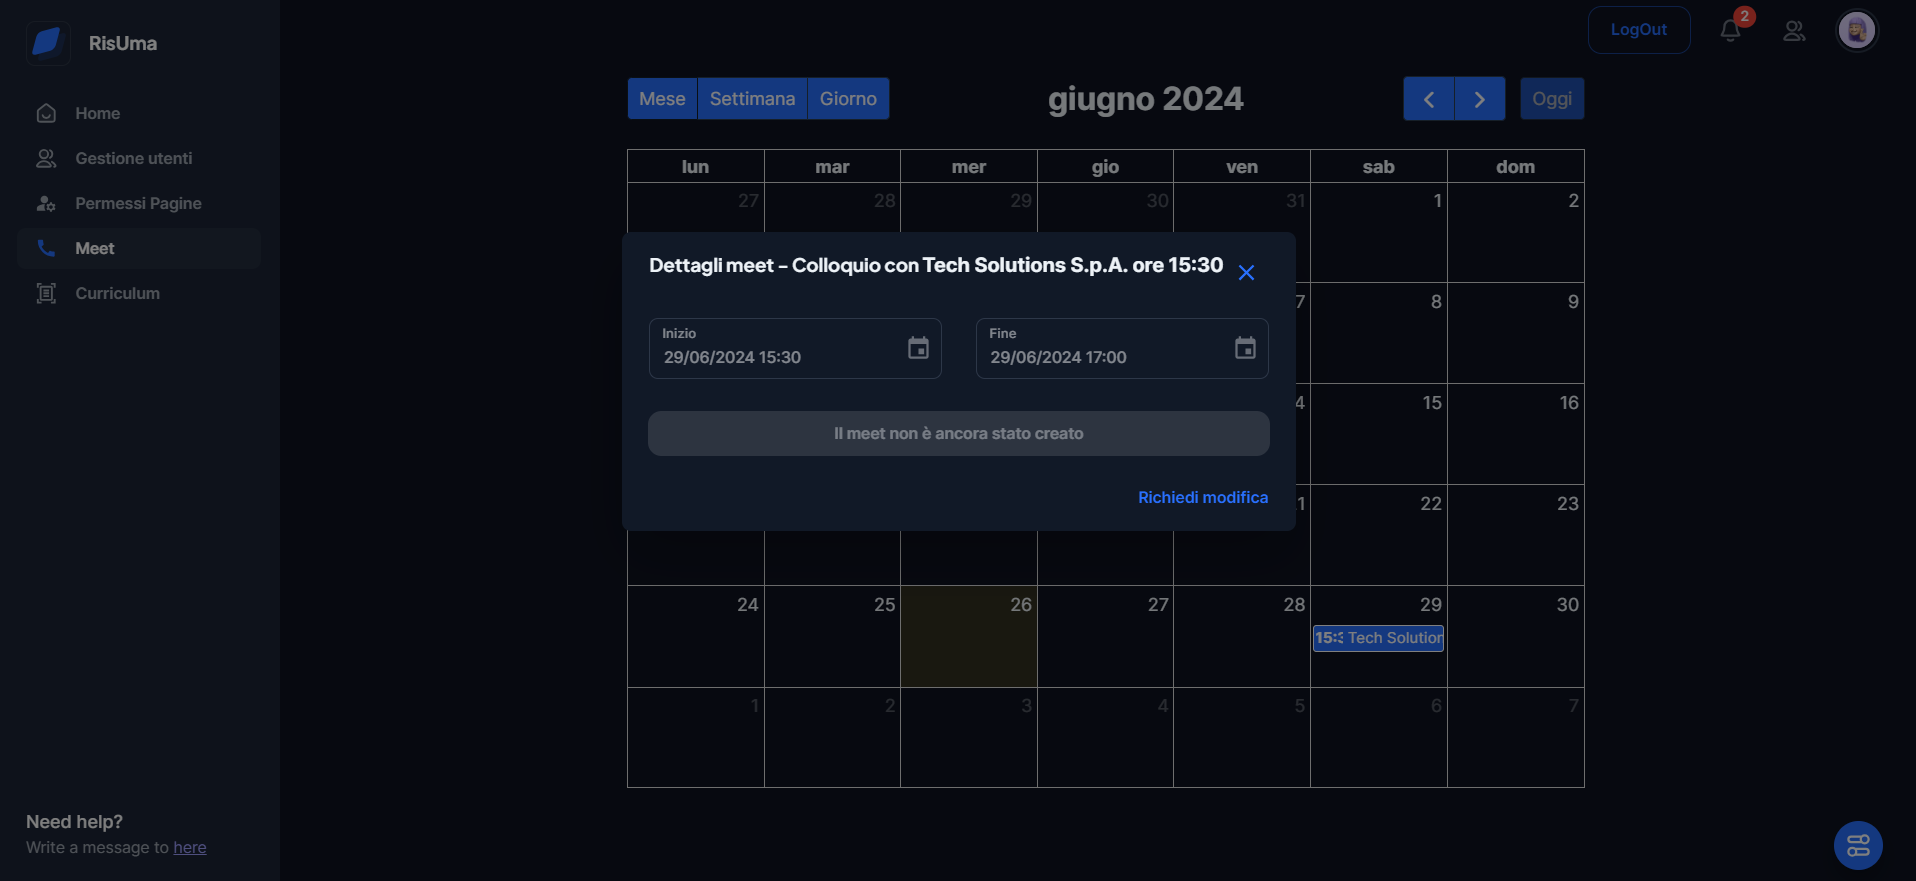
\includegraphics[width=\textwidth]{DettagliMeet/DettagliMeetUtente.png}
    \caption{Visualizzazione candidato - evento non iniziato}
\end{figure}
\begin{figure}[H]
    \centering
    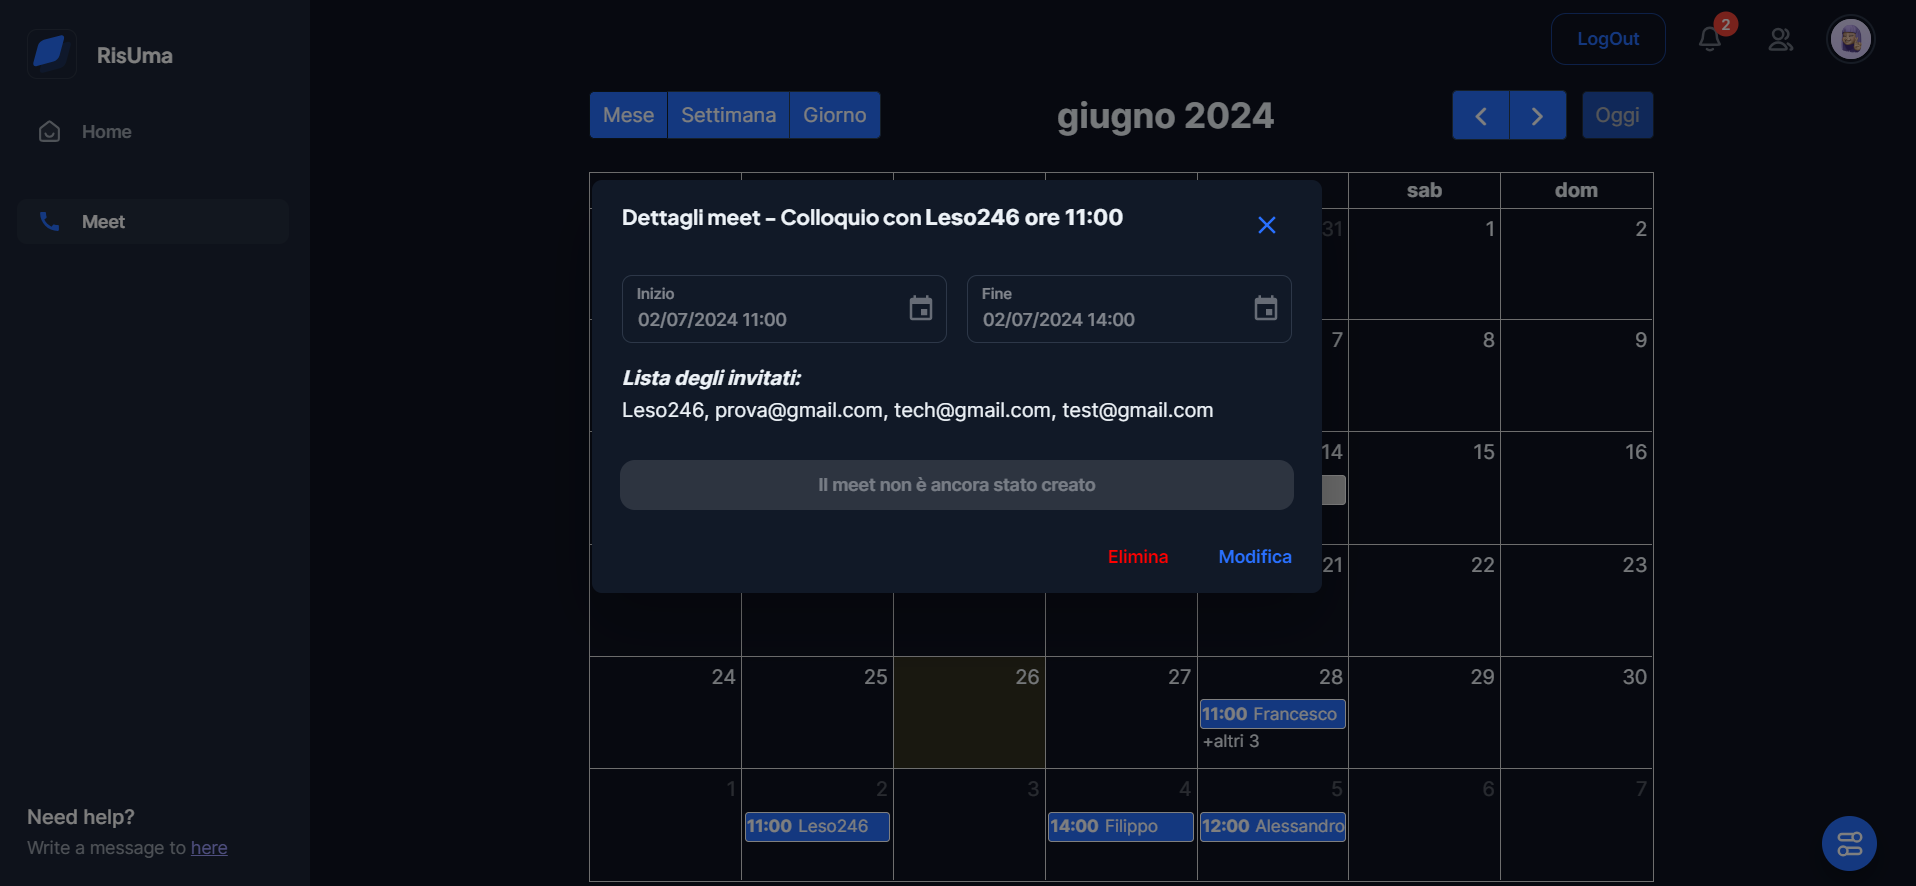
\includegraphics[width=\textwidth]{DettagliMeet/DettagliMeetAziendaDark.png}
    \caption{Visualizzazione azienda - evento non iniziato}
\end{figure}
\clearpage
\noindent Quando mancano meno di 10 minuti all'inizio del meet, il pulsante per partecipare 
al meet viene abilitato. Cliccandoci, si viene reinderizzati al meet su Webex.
In questo stato, l'evento non è più modificabile né eliminabile.
\begin{figure}[H]
    \centering
    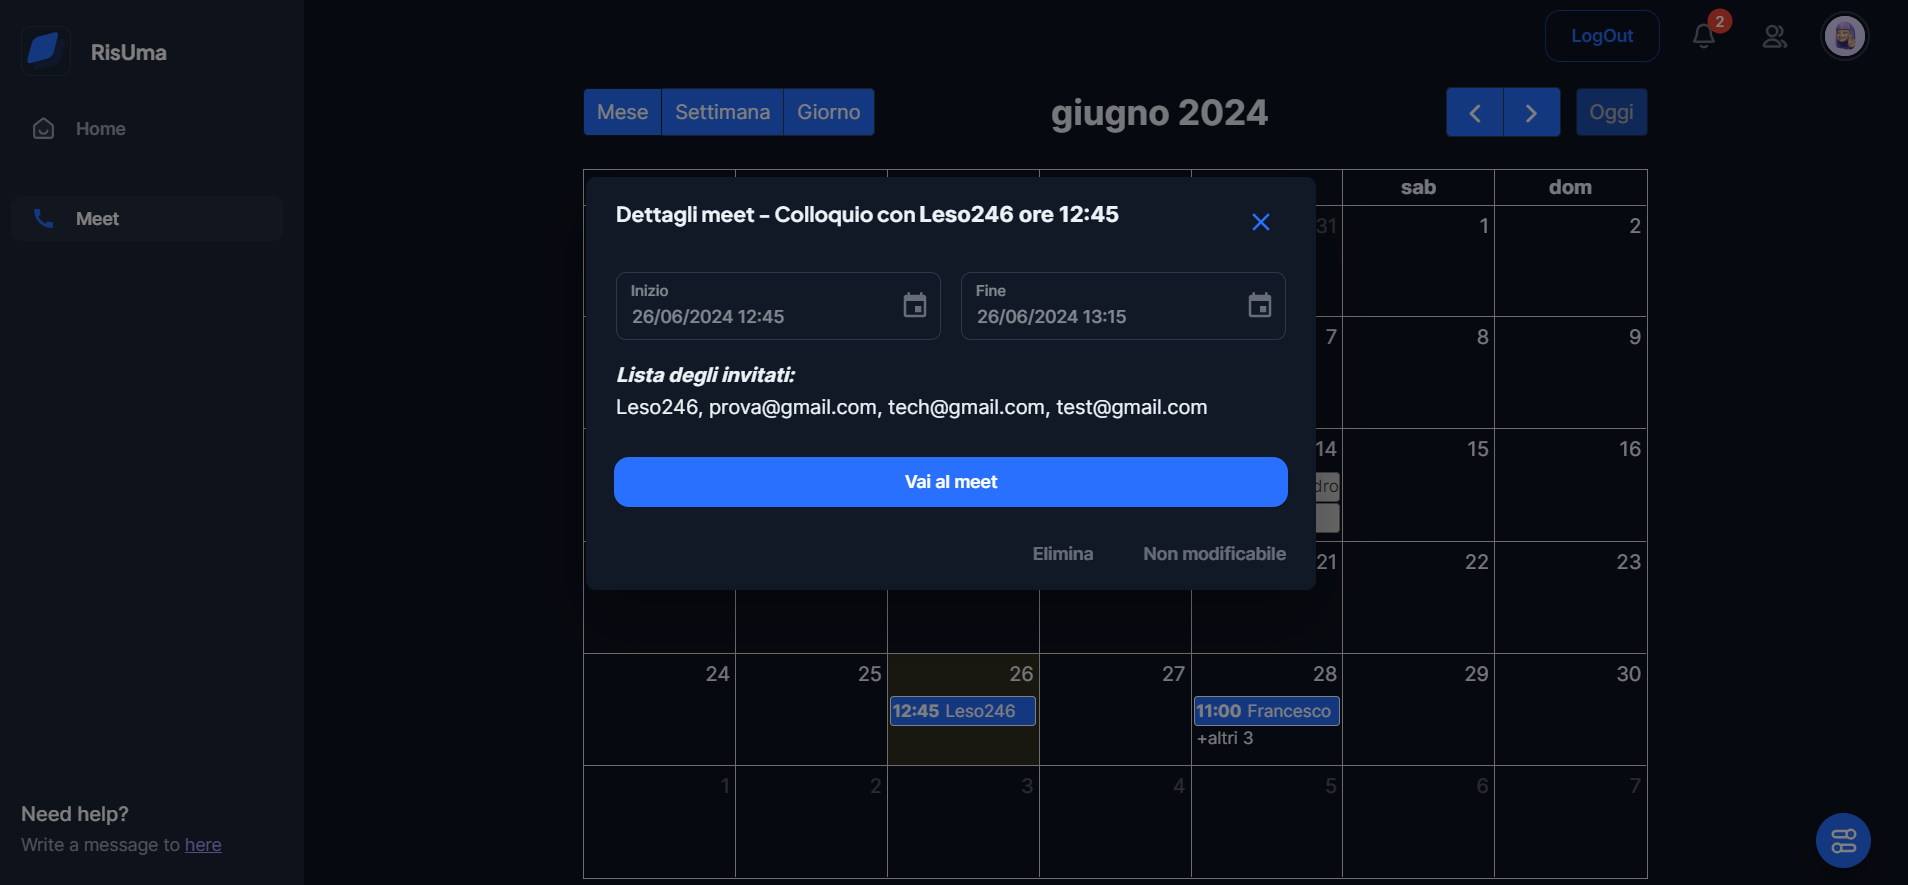
\includegraphics[width=\textwidth]{DettagliMeet/VaiAlMeet.png}
    \caption{Visualizzazione azienda - evento iniziato}
\end{figure}
\noindent Se l'evento è già concluso, è comunque possibile visualizzarne i dettagli 
per avere uno storico dell'incontro. In questo caso, non è possibile effettuare 
nessun'altra operazione sul meet.
\begin{figure}[H]
    \centering
    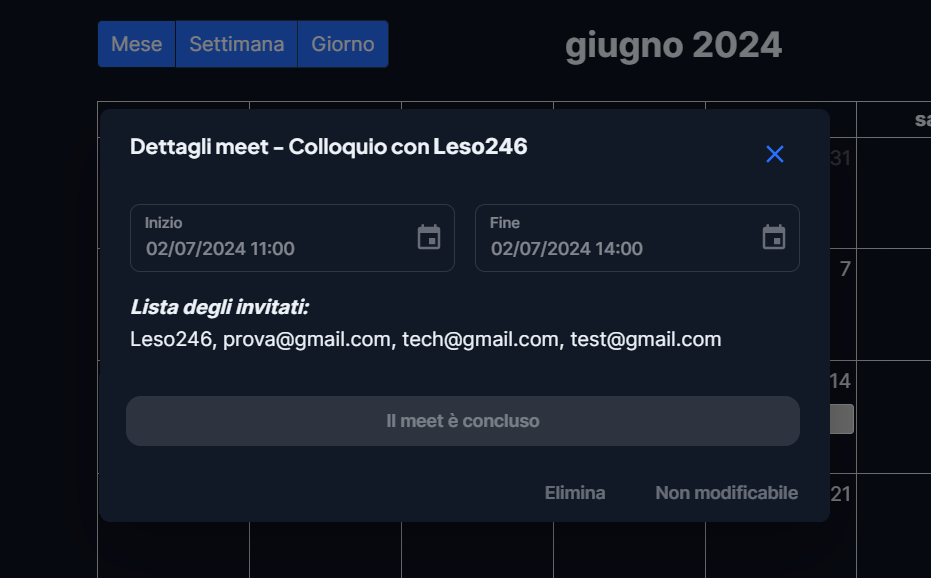
\includegraphics[width=\textwidth]{DettagliMeet/EventoConcluso.png}
    \caption{Visualizzazione azienda - evento concluso}
\end{figure}
\noindent La logica per abilitare/disabilitare i pulsanti è gestita interamente a frontend 
attraverso l'utilizzo di uno \texttt{useEffect}: ogni volta che un evento viene selezionato
e viene aperto il relativo \texttt{Dialog}, il sistema verifica la data attuale 
rispetto alla data di inizio e di fine del meeting. Questo controllo determina se mancano più di 10 
minuti all'inizio del meeting, se il meeting è già iniziato o se è concluso. Sulla base di questi valori, 
i pulsanti vengono abilitati o disabilitati di conseguenza.
\\ 
\\
È importante notare che al momento della creazione del meeting, 
l'orario di accesso per gli utenti è impostato 15 minuti prima della data di inizio. 
Questo permette di abilitare il pulsante "Vai al meet" in modo che gli utenti possano accedere 
direttamente senza attese o conferme.
\begin{lstlisting}[language=typescript, frame=lines, basicstyle=\ttfamily\scriptsize, numbers=left]
useEffect(() => {
    if (!selectedEvent) return;
      
    const { start, end } = selectedEvent;
    const now = new Date();
      
    const eventStartDate = new Date(start);
    const eventFinishDate = new Date(end);
      
    const minutesUntilStart = differenceInMinutes(eventStartDate, now);
    const isLessThan10Minutes = minutesUntilStart < 10;
    const isEventFinished = now > eventFinishDate;
      
    setIsLessThan10Minutes(isLessThan10Minutes);
    setIsEventFinished(isEventFinished);
}, [selectedEvent]);
\end{lstlisting}
\vspace{0.3cm}
Per quanto riguarda gli invitati a un meet, questi sono visualizzabili solo dall'azienda. 
Poiché non vengono salvati nel database, è necessario fare una chiamata all'API di Webex per recuperarli.
Considerato troppo oneroso effettuare una chiamata per ogni singolo meet durante il caricamento della 
pagina, l'API \texttt{/getMeetInvitees} viene chiamata ogni 
volta che si clicca su un evento. Sono stati effettuati 30 test e il tempo di risposta medio è 
risultato essere di 863 ms, motivo per cui questa soluzione è stata ritenuta adeguata. 
Prima che gli invitati vengano caricati, viene visualizzata 
una semplice scritta \textit{"Caricamento..."} di fianco alla dicitura \textit{"Lista degli invitati:"}
del \texttt{Dialog}.


\begin{lstlisting}[language=typescript, frame=lines, basicstyle=\ttfamily\scriptsize, numbers=left]
const handleEventClick = async (arg: any) => {
    setInvitees([]); // Resetta l'array di invitati
    setSelectedEvent(arg.event);
    setOpen(true); // Apre il Dialog 
    if (isAzienda) {
        const payload = {
        id: arg.event.id,
        webexId: arg.event.extendedProps.webexId,
        };
    
        try {
            const response = await getMeetInvitees(payload);
            if (response.status === 200) {
              setInvitees(response.data);
            } else {
              console.error('Errore nel recupero degli invitati:', response.statusText);
            }
          } catch (error) {
            console.error('Errore nel recupero degli invitati:', error);
          }
        }
    ...
\end{lstlisting}